\section{Data}
\label{sec:Data}
In order to enforce reproducibility of results, this section provides a detailed description of the generated synthetic datasets, as well as the real datasets, utilized in the results section.


\subsection{Synthetic Data}
\label{sec:Data:SyntheticData}
The synthetic data used for validating the SCVM is generated in order to be able to compare the learned model parameters with ground truth parameters.
The data is generated using the Poisson process simulation explained in detail under section \ref{sec:Method:PoissonSimulation}.

The ground truth parameters defined for each synthetic dataset are the number of nodes $N$, their initial positions $\textbf{Z}$, their initial velocities $\textbf{V}$ and the $\beta$ bias term.
One further parameter that has to be determined is the max time with which interactions are included, meaning interactions are simulated only for times $t < t_{max}$.


\subsubsection{Synthetic Dataset 1}
\label{sec:Data:SyntheticData:SyntheticDataset1}
The first synthetic dataset consists of four nodes, and will be utilized in order to evaluate the SCVM in a one step setting.
The ground truth parameters of the first synthetic dataset are as follows:
\begin{equation}
    N = 4, \hspace{10}
    t_{max} = 10, \hspace{10}
    \textbf{Z} = \left( \begin{matrix}
                -0.6 & 0.0\\
                0.6 & 0.1\\
                0.0 & 0.6\\
                0.0 & -0.6
                \end{matrix}\right), \hspace{10}
    \textbf{V} = \left( \begin{matrix}
                0.09 & 0.01\\
                -0.01 & -0.01\\
                0.01 & -0.09\\
                -0.01 & 0.09
                \end{matrix}\right), \hspace{10}
    \beta = 7.5
\end{equation}
These ground truth parameters yield a dataset, tuples denoting the two interacting nodes $u$ and $v$ in its first two columns, as well as the time of interaction $t$ in the third, ie. $(u_i, v_i, t_i)$, which has size $n=79,424$. 
The following links provide animations of the data:
\begin{align*}
    &\text{\bluehref{https://tgml-bachelor-project.github.io/GT-dataset1-no-correction.html}{LINK: SYNTHETIC DATASET 1 WITHOUT CORRECTION}} \\
    &\text{\bluehref{https://tgml-bachelor-project.github.io/GT-dataset1-with-correction.html}{LINK: SYNTHETIC DATASET 1 WITH CORRECTION}}
\end{align*}
to get a visual understanding of the setup.

\subsubsection{Synthetic Dataset 2}
\label{sec:Data:SyntheticData:SyntheticDataset2}
The second synthetic dataset is utilized in order to test the modelling capabilities of the SCVM on multi-step data. 

In order to generate a dataset which can properly showcase modelling using a stepwise approach, the velocities vectors associated with each node is changed over the timespan $(t_0, t_{max})$.
For synthetic dataset 2, five nodes are each attributed a starting position and 10 velocity vectors which each govern a tenth of the total time span.
The ground truth parameters of the second synthetic dataset are as follows:
\begin{equation}
    N = 5, \hspace{10}
    t_{max} = 50, \hspace{10}
    \textbf{Z} = \left( \begin{matrix}
                1 & 1\\
                1 & -1\\
                -1 & 1\\
                -1 & -1\\
                0 & 2
                \end{matrix}\right), \hspace{10}
    \textbf{V}_1 = \left( \begin{matrix}
                -0.15 & -0.15\\
                -0.15 & 0.15\\
                0.15 & -0.15\\
                0.15 & 0.15\\
                0.05 & -0.3
                \end{matrix}\right)... 
    \textbf{V}_{10} = \left( \begin{matrix}
                -0.15 & 0.05\\
                -0.15 & -0.05\\
                0.15 & -0.05\\
                0.15 & 0.05\\
                0.1 & 0.05
                \end{matrix}\right), \hspace{10}
    \beta = 7.5
\end{equation}
All velocity vectors are written in appendix \ref{appendix:SyntheticDataset2}.
\\
These ground truth parameters yield a dataset which has size $n=330,023$.
\\
To see an animated representation of the dataset the following links are provided:
\begin{align*}
    &\text{\bluehref{https://tgml-bachelor-project.github.io/GT-dataset2-no-correction.html}{LINK: SYNTHETIC DATASET 2 WITHOUT CORRECTION}} \\
    &\text{\bluehref{https://tgml-bachelor-project.github.io/GT-dataset2-with-correction.html}{LINK: SYNTHETIC DATASET 2 WITH CORRECTION}}
\end{align*}

\subsubsection{Synthetic Dataset 3}
\label{sec:Data:SyntheticData:SyntheticDataset3}
The third synthetic dataset is utilized in order to test scalability of the model, and for this purpose it is changeable in terms of number of nodes and beta value.
The number of nodes is chosen from the following range of $N$'s:
\begin{equation}
    N = [2, 4, 6, 8, 10, 12, 14, 16, 18, 20, 22, 24, 26, 28, 30, 34, 38, 42, 46, 50, 60]
\end{equation}
For the dataset consisting of $N = 2$ nodes, the starting positions are:
\begin{equation}
        \textbf{Z} = \left( \begin{matrix}
                1.0 & 0.0\\
                -1.0 & 0.0\\
                \end{matrix}\right)
\end{equation}
For the dataset consisting of $N = 6$ nodes, four more nodes are added which are placed further up along the y-axis, as the following:
\begin{equation}
        \textbf{Z} = \left( \begin{matrix}
                1.0 & 0.0\\
                -1.0 & 0.0\\
                1.0 & 1.0\\
                -1.0 & 1.0\\
                1.0 & 2.0\\
                -1.0 & 2.0\\
                \end{matrix}\right)
\end{equation}
The nodes in these starting positions look as presented on figure \ref{fig:synth3}.
\begin{figure}[H]
    \centering
    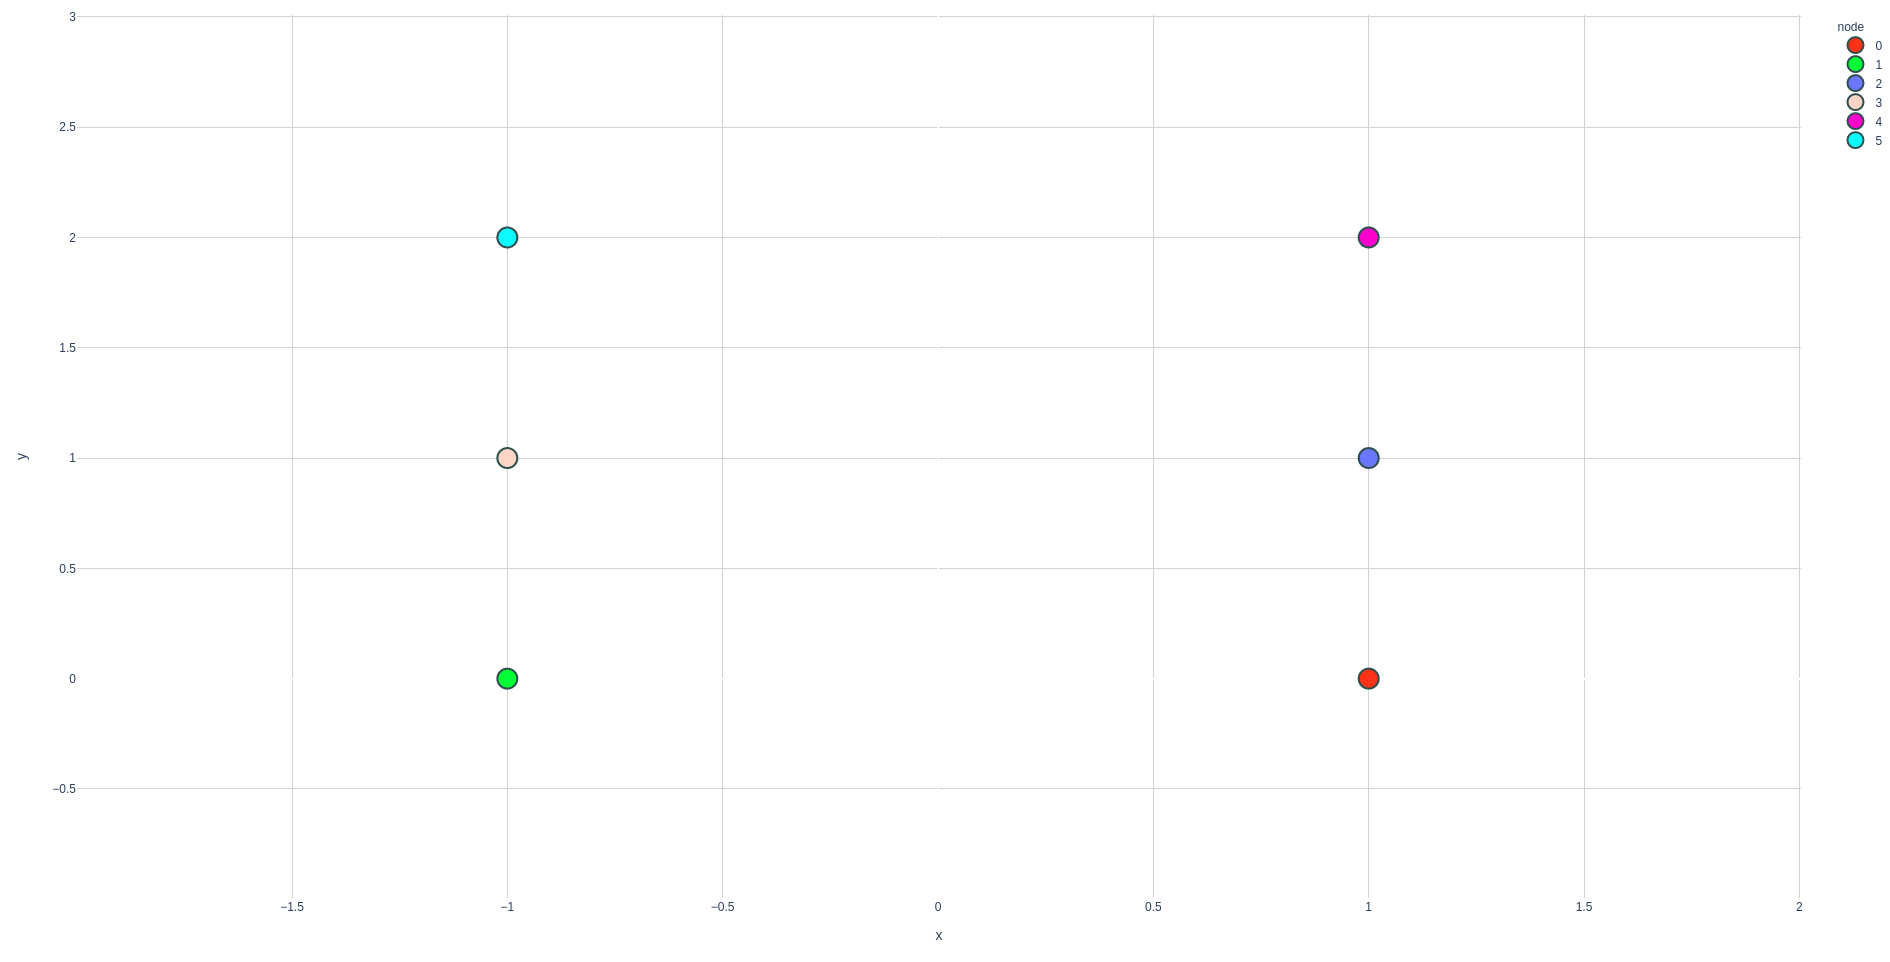
\includegraphics[width=\textwidth]{0_images/synth3_n6.png}
    \caption{Synthetic dataset 3 with $N=6$ nodes at $t_0$.}
    \label{fig:synth3}
\end{figure}

\noindent The beta value $\beta$ is, like the number of nodes, also chosen from a range as follows:

\begin{equation}
    \beta = [5.0, 5.25, 5.5, 5.75, 6.0, 6.25, 6.5, 6.75, 7.0, 7.25, 7.5, 7.75, 8.0, 8.25, 8.5, 8.75, 9.0]
\end{equation}
The max time is $t_{max} = 20$, and as such the remaining ground truth parameter of the third synthetic dataset are the velocities of the four steps, which are replicated for each added set of nodes:
\begin{equation}
    
    V_1 = \left( \begin{matrix}
                -0.2 & -0.05\\
                0.2 & 0.05\\
                \end{matrix}\right), \hspace{5}
    V_2 = \left( \begin{matrix}
                0.2 & 0.05\\
                -0.2 & -0.05\\
                \end{matrix}\right), \hspace{5}
    V_3 = \left( \begin{matrix}
                -0.3 & -0.05\\
                0.3 & 0.05\\
                \end{matrix}\right), \hspace{5}
    V_4 = \left( \begin{matrix}
                0.3 & 0.05\\
                -0.3 & -0.05\\
                \end{matrix}\right)
\end{equation}
A visual representation is provided through the links below:
\begin{align*}
    &\text{\bluehref{https://tgml-bachelor-project.github.io/GT-dataset3-no-correction.html}{LINK: SYNTHETIC DATASET 3 WITHOUT CORRECTION}} \\
    &\text{\bluehref{https://tgml-bachelor-project.github.io/GT-dataset3-with-correction.html}{LINK: SYNTHETIC DATASET 3 WITH CORRECTION}}
\end{align*}

\subsection{Real Data}
\label{sec:Data:RealData}


\subsubsection{Real Dataset 1: Player Interactions in a game of 'Resistance'}
\label{sec:Data:RealData:RealDataset1}
Dataset can be found here:
\\
\href{https://snap.stanford.edu/data/comm-f2f-Resistance.html}{https://snap.stanford.edu/data/comm-f2f-Resistance.html}
\\\\
The first real dataset consists of player interactions in a game of Resistance. 
This dataset has been chosen, at is one of few temporally dynamic networks available, which has relatively few nodes yet still many interactions.
\\
The Resistance game is a discussion, find-the-fraudster game, in which each player has a role belonging to either the resistance (good guys) or government spies (evil guys).
Only the government spies know the identity of their teammates, and so the goal of the game is for the resistance to identify the spies through verbal communication and vote them out, while the spies try to vote out the resistance by acting innocence. 
\\
The interactions that make up the dataset are synthesized from a video recording of one such game of Resistance.
For each time point, every third of a second, a perception algorithm, \cite{BaiPredictingVideos} \cite{Kumar2019PredictingNetworks}, evaluates for every player which other player he or she is most likely to be looking at.
For utilizing this dataset in the project, one player looking at another player is defined as an interaction between the two.
\\
The specific dataset, game 4 of the included 62 games in the overall dataset, has eight players and a computer with which the players can interact to get hints during the game.
This makes for $N=9$ nodes, having a total of 58.584 interactions spanning from time $t_{0} = 0$ seconds to $t_{max} = 2440$ seconds, approximately $40$ minutes and $40$ seconds.
The timestamps are transformed from thirds of a second to minutes by the following formula:

\begin{equation}
    t_i = 40.67 \cdot \frac{t_i - t_{min}}{t_{max}}
\end{equation}
The overall distribution of interactions are completely uniformly distributed due to the recording process.



\subsubsection{Real Dataset 2: Student interactions in Lyon Primary School}
\label{sec:Data:RealData:RealDataset3}
Dataset can be found here: \href{http://www.sociopatterns.org/datasets/co-location-data-for-several-sociopatterns-data-sets/}{http://www.sociopatterns.org/datasets/co-location-data-for-several-sociopatterns-data-sets/}
\\\\
The second real dataset consists of co-location data of the students and teachers of a primary school in Lyon, France.
The original dataset consists of 241 individuals with 6.594.492, 20-second co-locations, meaning face-to-face presence that persist over the span of 20 seconds, which serve as the interactions of the dataset.
The first interactions happening at $t_{0} = 34,240$ seconds and the last at 151.960 seconds.
The data is essentially split temporally in two, and around half of interactions, 3.510.605, happen before time $t_{max} = 65,840$ seconds.
The dataset used for the project is this first half, consisting of $N = 237$ nodes with $n = 3,510,605$ interactions.
%From this half, the $n = 958,220$ interactions of 98 students and teachers are utilized.
The timestamps are transformed to hours, starting at hour 0 and ending at 84.25, by the following formula:

\begin{equation}
    t_i = \left(\frac{t_{max} - t_{min}}{3 \cdot 60} \right) \cdot \frac{t_i - t_{min}}{t_{max}}
\end{equation}
The interaction of the Lyon primary School dataset have the distribution shown in figure \ref{fig:RLdataset3} below:

\begin{figure}[H]
    \centering
    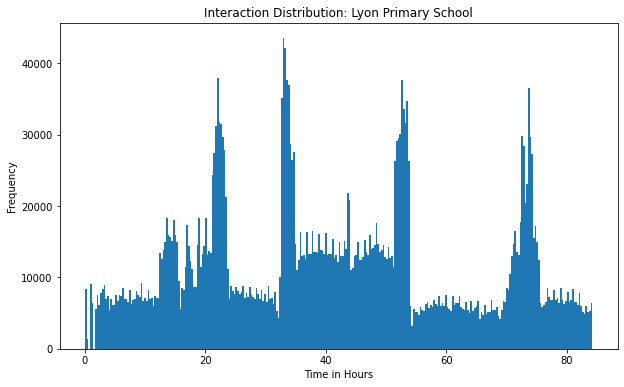
\includegraphics[width=\textwidth]{0_images/real_dataset_3_dist.png}
    \caption{Distribution of Real Dataset 2: Lyon Primary School}
    \label{fig:RLdataset3}
\end{figure}







